% to be compiled with: pdflatex --jobname=profile-f1 profile.tex
\documentclass[12pt]{book}
\usepackage[utf8]{inputenc}
\usepackage[T1]{fontenc}
\usepackage[frenchstyle,fulloldstylenums,partialup]{kpfonts}
\usepackage{tikz}
\usetikzlibrary{snakes}
%\pgfrealjobname{profile}
\begin{document}
\beginpgfgraphicnamed{profile-f1}
\footnotesize
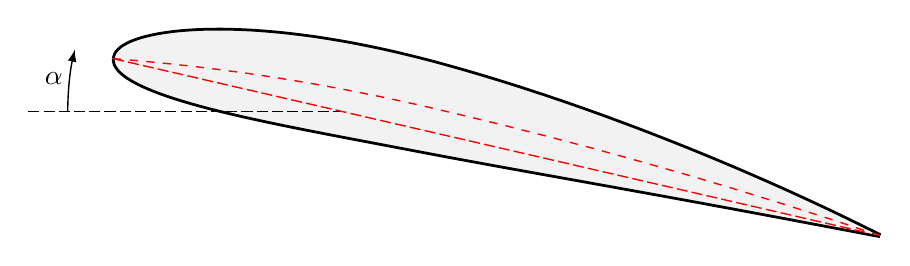
\begin{tikzpicture}[>=latex,scale=1]
\tikzstyle{spring}=[snake=zigzag,thick,line before snake=0.3cm,line after  snake=0.3cm,segment length=6,segment amplitude=5,join=round]%
\begin{scope}[rotate around={-13:(10,0)}]
% bottom_second
\draw[smooth,line width=1pt,fill=black!5] plot coordinates {(0,0)(0.0334,-0.0767)(0.1087,-0.1437)(0.2253,-0.2011)(0.3824,-0.2489)(0.5790,-0.2870)(0.8139,-0.3158)(1.0860,-0.3355)(1.3940,-0.3466)(1.7365,-0.3497)(2.1123,-0.3457)(2.5199,-0.3356) (2.9580,-0.3209)(3.4252,-0.3029)(3.9198,-0.2835)(4.4427,-0.2625)(4.9936,-0.2377)(5.5666,-0.2102)(6.1594,-0.1810)(6.7696,-0.1513)(7.3950,-0.1217)(8.0332,-0.0930)(8.6815,-0.0653)(9.3376,-0.0386)(9.9988,-0.0125)};
% top_first
\draw[smooth,line width=1pt,fill=black!5] plot coordinates {(0,0)(0.0095,0.0831)(0.0624,0.1691)(0.1590,0.2574)(0.2990,0.3467)(0.4824,0.4357)(0.7085,0.5225)(0.9765,0.6050)(1.2855,0.6812)(1.6341,0.7488)(2.0206,0.8055)(2.4433,0.8492)(2.8998,0.8778)(3.3879,0.8897)(3.9049,0.8833)(4.4459,0.8592)(5.0064,0.8210)(5.5876,0.7687)(6.1870,0.7023)(6.8016,0.6219)(7.4286,0.5277)(8.0650,0.4197)(8.7080,0.2980)(9.3544,0.1623)(10.0012,0.0125)};
% sekelett
\draw[dashed, color=red, line width=0.5pt,fill=black!5] plot coordinates { (0.0, 0.0)(0.021, 0.003)(0.086, 0.013)(0.192, 0.028)(0.341, 0.049)(0.531, 0.074)(0.761, 0.103)(1.031, 0.135)(1.34, 0.167)(1.685, 0.2)(2.066, 0.23)(2.482, 0.257)(2.929, 0.278)(3.407, 0.293)(3.912, 0.3)(4.444, 0.298)(5.0, 0.292)(5.577, 0.279)(6.173, 0.261)(6.786, 0.235)(7.412, 0.203)(8.049, 0.163)(8.695, 0.116)(9.346, 0.062)(10.0, 0.0) };
\draw[line width=0.5pt,dashed,dash pattern=on 4pt off 1.5pt,rotate around={13:(3,0)}](-1,0)--(3,0);
% arrows
\draw[line width=0.5pt,<-](3,0) +(180:3.5cm) arc (180:193:3.5cm);
\draw(3,0) +(186.5:3.7cm) node{$\alpha$};
% sehne
\draw[line width=0.5pt,color=red, dashed,dash pattern=on 4pt off 1.5pt](0,0)--(9.8,0);
\end{scope}%
\end{tikzpicture}
\endpgfgraphicnamed%
\end{document}